\section{Pooling auf Graphen}
\label{pooling}

Neben den Faltungsschichten gehören die sogenannten Poolingschichten zu den fundamentalen Schichten eines \glspl{CNN}.
Poolingschichten eines Netzes, üblicherweise über Max-Pooling realisiert, werden dabei für gewöhnlich direkt nach einer Faltungsschicht benutzt und sorgen dafür, die Ausgabe der Faltung zu filtern \bzw{} zu reduzieren~\cite{Nielsen}.

Eine Pooling-Operation auf Graphen erfordert dafür analog zum Pooling auf einem regulären Gitter eine logische Zusammenfassung von Knoten zu Clustern~\cite{Defferrard}.
Der zu verwendende Clusteralgorithmus hat dabei jedoch einige Anforderungen, um als Poolingoperation in einem Netz genutzt werden zu könnnen.
So muss dieser vor allem als ein mehrstufiges Clustering fungieren, bei dem jede Stufe eines Graphen den Blick auf den Graphen bei einer unterschiedlichen \enquote{Auflösung} zeigt und insbesondere die zugrunde liegende Geometrie des Graphen erhält~\cite{Defferrard}.
Das Clustering von Knoten wird daher in dieser Arbeit auch oft als \emph{Vergröberung} eines Graphen betitelt.
Die mehrfache Anwendung eines Clusteralgorithmus erlaubt damit die mehrfache Benutzung von Poolingschichten im Netz.
Es ist weiterhin notwendig, dass die Poolingoperation benutzerspezifische Poolinggrößen ermöglicht.
Hier erscheinen vor allem Clustertechniken sinnvoll, die die Größe eines Graphen um den Faktor zwei reduzieren~\cite{Defferrard}.
Damit können größere Poolinggrößen über die mehrfache Anwendung des Clusteralgorithmus realisiert werden.

\subsection{Graphvergröberung}
\label{graphvergroeberung}

Es existiert eine Reihe von Clustertechniken auf Graphen~\cite{Luxburg, graclus, Defferrard}.
\citeauthor{Defferrard} benutzen für die Poolingschicht eines Netzes auf Graphen die \emph{Vergröberungsphase} des mehrstufigen Clusteralgorithmus \emph{Graclus}~\cite{graclus}.
Graclus zeigt sich dabei als besonders erfolgreich über einer Vielzahl von Graphen bei minimaler Berechnungskomplexität~\cite{Defferrard}.
Abbildung~\ref{fig:clustering} illustriert den Ablauf des Algorithmus.
\begin{figure}[t]
\centering
\subfigure[Graph mit zufälliger Ordnung]{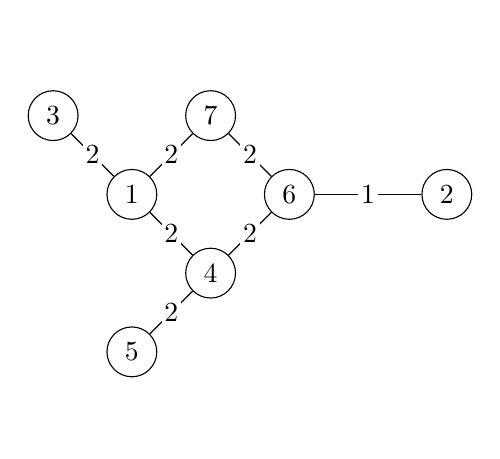
\begin{tikzpicture}
  \fill [white] (-3, -3) rectangle (2, 2) node {};  % Zentriere Graph.
  \tikzstyle{node}=[circle,draw, minimum width=18pt, inner sep=0pt, fill=white]
  \tikzstyle{label}=[fill=white, inner sep=1pt]

  \node[node] (1) at (-3, 1)  {$3$};
  \node[node] (2) at (-2, 0)  {$1$};
  \node[node] (3) at (-1, 1)  {$7$};
  \node[node] (4) at (-1, -1) {$4$};
  \node[node] (5) at (0, 0)   {$6$};
  \node[node] (6) at (-2, -2) {$5$};
  \node[node] (7) at (2, 0)   {$2$};

  \path (1) edge node[label] {$2$} (2);
  \path (2) edge node[label] {$2$} (3);
  \path (2) edge node[label] {$2$} (4);
  \path (3) edge node[label] {$2$} (5);
  \path (4) edge node[label] {$2$} (5);
  \path (4) edge node[label] {$2$} (6);
  \path (5) edge node[label] {$1$} (7);
\end{tikzpicture}
}
\hspace{1cm}
\subfigure[Bestimmung des Normalized-Cuts]{\begin{tabular}[b]{ccc}
  \toprule
  Kante & Gewicht & Normalized-Cut\\
  \toprule
  $\left(1,3\right)$ & 2 & $\mathbf{1.\overline{3}}\,\,\,$\\
  $\left(1,4\right)$ & 2 & $0.\overline{3}\,\,\,$\\
  $\left(1,7\right)$ & 2 & $0.8\overline{3}$\\
  \midrule
  $\left(2,6\right)$ & $1$ & $\mathbf{1.2}\,\,\,$\\
  \midrule
  $\left(4,5\right)$ & $2$ & $\mathbf{1.\overline{3}}\,\,\,$\\
  $\left(4,6\right)$ & $2$ & $0.7\overline{3}$\\
  \midrule
  $\left(6,7\right)$ & $2$ & $\mathbf{0.9}\,\,\,$\\
  \bottomrule
\end{tabular}
}
\hspace{1cm}
\subfigure[Clustering der Knoten]{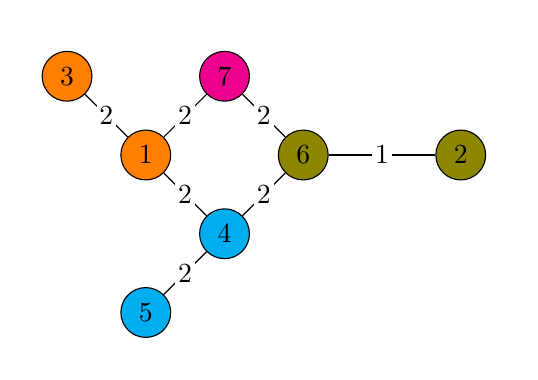
\begin{tikzpicture}
  \fill [white] (-3.5, -2.5) rectangle (2.5, 1.5) node {};  % Zentriere Graph.
  \tikzstyle{node}=[circle,draw, minimum width=18pt, inner sep=0pt, fill=white]
  \tikzstyle{color1}=[fill=orange]
  \tikzstyle{color2}=[fill=olive]
  \tikzstyle{color3}=[fill=cyan]
  \tikzstyle{color4}=[fill=magenta]
  \tikzstyle{label}=[fill=white, inner sep=1pt]

  \node[node, color1] (1) at (-3, 1)  {$3$};
  \node[node, color1] (2) at (-2, 0)  {$1$};
  \node[node, color4] (3) at (-1, 1)  {$7$};
  \node[node, color3] (4) at (-1, -1) {$4$};
  \node[node, color2] (5) at (0, 0)   {$6$};
  \node[node, color3] (6) at (-2, -2) {$5$};
  \node[node, color2] (7) at (2, 0)   {$2$};

  \path (1) edge node[label] {$2$} (2);
  \path (2) edge node[label] {$2$} (3);
  \path (2) edge node[label] {$2$} (4);
  \path (3) edge node[label] {$2$} (5);
  \path (4) edge node[label] {$2$} (5);
  \path (4) edge node[label] {$2$} (6);
  \path (5) edge node[label] {$1$} (7);
\end{tikzpicture}
}
\hspace{1cm}
\subfigure[vergröberter Graph]{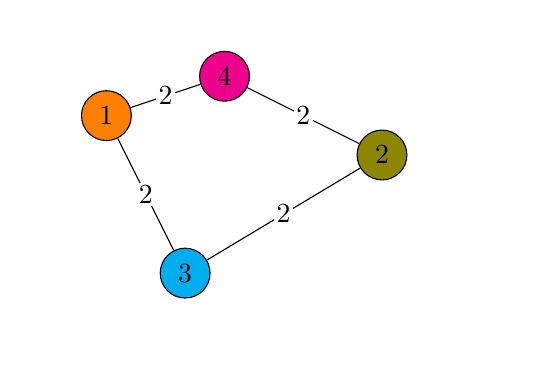
\begin{tikzpicture}
  \fill [white] (-3.5, -2.5) rectangle (2.5, 1.5) node {};  % Zentriere Graph.

  \tikzstyle{node}=[circle,draw, minimum width=18pt, inner sep=0pt, fill=white]
  \tikzstyle{color1}=[fill=orange]
  \tikzstyle{color2}=[fill=olive]
  \tikzstyle{color3}=[fill=cyan]
  \tikzstyle{color4}=[fill=magenta]
  \tikzstyle{label}=[fill=white, inner sep=1pt]

  \node[node, color1] (1) at (-2.5, 0.5)  {$1$};
  \node[node, color2] (2) at (1, 0)       {$2$};
  \node[node, color3] (3) at (-1.5, -1.5) {$3$};
  \node[node, color4] (4) at (-1, 1)      {$4$};

  \path (1) edge node[label] {$2$} (3);
  \path (1) edge node[label] {$2$} (4);
  \path (2) edge node[label] {$2$} (3);
  \path (2) edge node[label] {$2$} (4);
\end{tikzpicture}
}
\caption[Graphvergröberung mittels Graclus und Normalized-Cut]{Vergröberung eines Graphen \gls{G} mittels Graclus und Normalized-Cut bei zufälliger Knotenordung, hier angegeben über die Knotenindizes von \gls{G} (a).
Die Maxima des Normalized-Cuts (b) zwischen den Knoten und deren lokalen Nachbarschaften bestimmen in aufsteigender Reihenfolge das höchstens paarweise Clustering von \gls{V} (c).
Der vergröberte Graph ergibt sich dann als clusterweise Aufsummierung der Kanten ohne Schleifen (d).}
\label{fig:clustering}
\end{figure}

Dabei wird ein initialer Graph $\gls{G}_0$ sukzessive in kleinere Graphen $\gls{G}_1, \gls{G}_2, \ldots, \gls{G}_L$ mit $\left|\gls{V}_0\right| > \left|\gls{V}_1\right| > \cdots > |\gls{V}_L|$, $L \in \gls{N}$, transformiert~\cite{graclus}.
Für die Transformation von einem Graphen $\gls{G}_l$ zu einem Graphen $\gls{G}_{l+1}$ mit kleinerer Knotenanzahl $\left|\gls{V}_{l+1}\right| < \left|\gls{V}_l\right|$ werden aus disjunkten Knotenuntermengen von $\gls{V}_l$ \emph{Superknoten} für $\gls{V}_{l+1}$ gebildet~\cite{graclus}.
Die Kantengewichte $\gls{E}_{l+1}$ werden dann über die Summe der Kantengewichte der jeweiligen Knotenuntermengen ohne Schleifen gebildet~\cite{graclus}.

Die Auswahl der Untermengen erfolgt gierig.
Die Knoten des Graphen $\gls{G}_l$ werden als unmarkiert initialisert und zufällig durchlaufen.
Für jeden Knoten $\gls{v}_i \in \gls{V}_l$, der noch unmarkiert ist, wird ein lokaler, ebenfalls noch unmarkierter, Nachbarschaftsknoten $\gls{v}_j \in \gls{Neighbor}\left(\gls{v}_i\right)$ nach einer zuvor definierten Strategie bestimmt und $\gls{v}_i$ sowie $\gls{v}_j$ zu einem Superknoten $\gls{v}^* \coloneqq \left\{ \gls{v}_i, \gls{v}_j \right\} \in \gls{V}_{l+1}$ verschmolzen.
Anschließend werden $\gls{v}_i$ sowie $\gls{v}_j$ markiert.
Falls $\gls{v}_i$ keinen unmarkierten Nachbarknoten besitzt, wird $\gls{v}_i$ alleine als Superknoten $\gls{v}^* \coloneqq \left\{ \gls{v}_i \right\} \in \gls{V}_{l+1}$ deklariert und markiert.
Der Algorithmus ist abgeschlossen, sobald alle Knoten erfolgreich markiert wurden~\cite{graclus}.
Bei weiteren Anwendungen des Clusteralgorithmus werden die Knoten im Folgenden anhand ihrer aufsteigenden Knotengrade durchlaufen~\cite{Defferrard}.

Strategien für die Nachbarschaftsauswahl basieren üblicherweise auf der Maximierung von $\gls{w}\left(\gls{v}_i, \gls{v}_j \right)$~\cite{graclus}.
Eine darauf aufbauende Strategie ist der \emph{Normalized-Cut}
\begin{equation*}
  \gls{ncut}\left(\gls{v}_i, \gls{v}_j\right) \coloneqq \gls{w}\left(\gls{v}_i, \gls{v}_j \right) \left(\frac{1}{\gls{d}\left(\gls{v}_i\right)} + \frac{1}{\gls{d}\left(\gls{v}_j\right)}\right),
\end{equation*}
der die Kantengewichte relativ zu ihrem Knotengrad gewichtet~\cite{Defferrard, graclus}.
Der Nor\-ma\-li\-zed-Cut sorgt dafür, dass Kanten als wichtiger gezählt werden, wenn ihre entsprechenden Knoten einen geringen Grad besitzen und damit folglich als unwahrscheinlicher gelten, mit einem anderen Knoten zu verschmelzen.

Graclus reduziert die Knotenanzahl eines beliebigen Graphen näherungsweise um die Hälfte, \dhe{} $2 \left|\gls{V}_{l+1}\right| \approx \left|\gls{V}_l\right|$.
Es können jedoch vereinzelt Superknoten entstehen, die nur aus einem einzigen Knoten der vorangegangenen Schicht gebildet wurden.
In der Praxis zeigt sich jedoch, dass Graclus nur sehr wenige solcher Superknoten generiert~\cite{Defferrard}.
Es ist weiterhin wichtig anzumerken, dass der Algorithmus bei mehrmaliger Anwendung auf dem gleichen Graphen aufgrund seiner zufälligen Iteration auf den Knoten zwei verschiedene, vergröberte Graphen erzeugen kann.
Damit kann der Prozess des Clusterings bereits als ein Augmentierungsschritt der Eingabedaten verstanden werden.

\subsection{Effizientes Pooling mittels binärer Bäume}
\label{pooling_mit_baeumen}

Ein tiefes neuronales Netz besitzt für gewöhnlich viele Poolingschichten.
Eine Poo\-ling-Operation auf den Merkmalen der Graphknoten muss folglich vor allem effizient sein.
Ein naiver Ansatz dafür ist eine \emph{Lookup-Tabelle}, in der die Verbindungen der Knoten zu ihren Superknoten gespeichert sind.
Eine Poolingoperation muss demnach für jedes Cluster ihre Knoten in der Tabelle referenzieren und ihre Operation auf diesen vollführen.
Das resultiert in einer extrem speicherineffizienten, langsamen und schwer zu parallelisierenden Implementierung~\cite{Defferrard}.
Es ist jedoch möglich, die Knoten des Graphen so anzuordnen, dass eine Poolingoperation auf diesen in linearer Zeit, \dhe{} $\gls{O}\left(N\right)$, realisiert werden kann~\cite{Defferrard}.

\begin{figure}[t]
\centering
  \subfigure[$\gls{G}_0$]{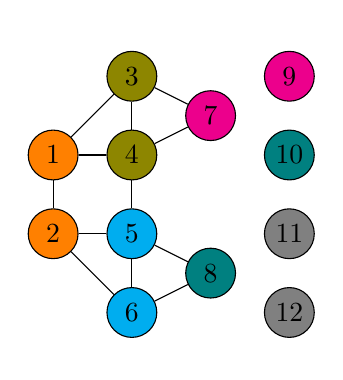
\begin{tikzpicture}
  \fill [white] (-1, -2) rectangle (1, 2) node {};  % Zentriere Graph.
  \tikzstyle{node}=[circle,draw, minimum width=18pt, inner sep=0pt, fill=white]
  \tikzstyle{color1}=[fill=orange]
  \tikzstyle{color2}=[fill=olive]
  \tikzstyle{color3}=[fill=cyan]
  \tikzstyle{color4}=[fill=magenta]
  \tikzstyle{color5}=[fill=teal]
  \tikzstyle{color6}=[fill=gray]

  \node[node, color1] (1)  at (-2, 0.5)  {$1$};
  \node[node, color1] (2)  at (-2, -0.5) {$2$};
  \node[node, color2] (3)  at (-1, 1.5)  {$3$};
  \node[node, color2] (4)  at (-1, 0.5)  {$4$};
  \node[node, color3] (5)  at (-1, -0.5) {$5$};
  \node[node, color3] (6)  at (-1, -1.5) {$6$};
  \node[node, color4] (7)  at (0,  1)    {$7$};
  \node[node, color5] (8)  at (0,  -1)   {$8$};

  \node[node, color4] (9)  at (1, 1.5)   {$9$};
  \node[node, color5] (10) at (1, 0.5)   {$10$};
  \node[node, color6] (11) at (1, -0.5)  {$11$};
  \node[node, color6] (12) at (1, -1.5)  {$12$};

  \path (1) edge (2);
  \path (1) edge (3);
  \path (1) edge (4);
  \path (2) edge (5);
  \path (2) edge (6);
  \path (3) edge (4);
  \path (3) edge (7);
  \path (4) edge (5);
  \path (4) edge (7);
  \path (5) edge (6);
  \path (5) edge (8);
  \path (6) edge (8);
\end{tikzpicture}
}
\hspace{1cm}
  \subfigure[$\gls{G}_1$]{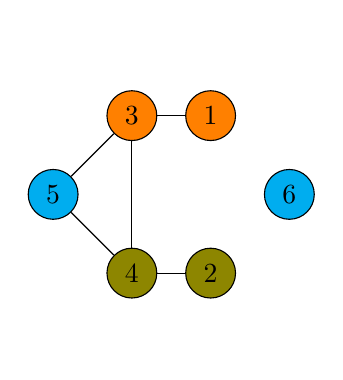
\begin{tikzpicture}
  \fill [white] (-1, -2) rectangle (1, 2) node {};  % Zentriere Graph.
  \tikzstyle{node}=[circle,draw, minimum width=18pt, inner sep=0pt, fill=white]
  \tikzstyle{color1}=[fill=orange]
  \tikzstyle{color2}=[fill=olive]
  \tikzstyle{color3}=[fill=cyan]

  \node[node, color3] (1) at (-1, 0) {$5$};
  \node[node, color1] (2) at (0,  1) {$3$};
  \node[node, color2] (3) at (0, -1) {$4$};
  \node[node, color1] (4) at (1,  1) {$1$};
  \node[node, color2] (5) at (1, -1) {$2$};

  \node[node, color3] (6) at (2, 0)  {$6$};

  \path (1) edge (2);
  \path (1) edge (3);
  \path (2) edge (3);
  \path (2) edge (4);
  \path (3) edge (5);
\end{tikzpicture}
}
\hspace{1cm}
  \subfigure[$\gls{G}_2$]{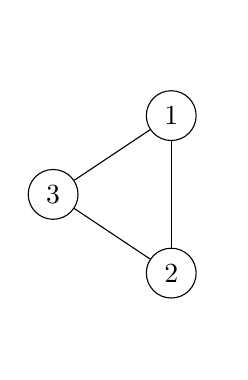
\begin{tikzpicture}
  \fill [white] (-1, -2) rectangle (1, 2) node {};  % Zentriere Graph.
  \tikzstyle{node}=[circle,draw, minimum width=18pt, inner sep=0pt, fill=white]

  \node[node] (1) at (-1,   0) {$3$};
  \node[node] (2) at (0.5,  1) {$1$};
  \node[node] (3) at (0.5, -1) {$2$};

  \path (1) edge (2);
  \path (1) edge (3);
  \path (2) edge (3);
\end{tikzpicture}
}
\hspace{1cm}
  \subfigure[Anorderung der Knoten zu einem binären Baum]{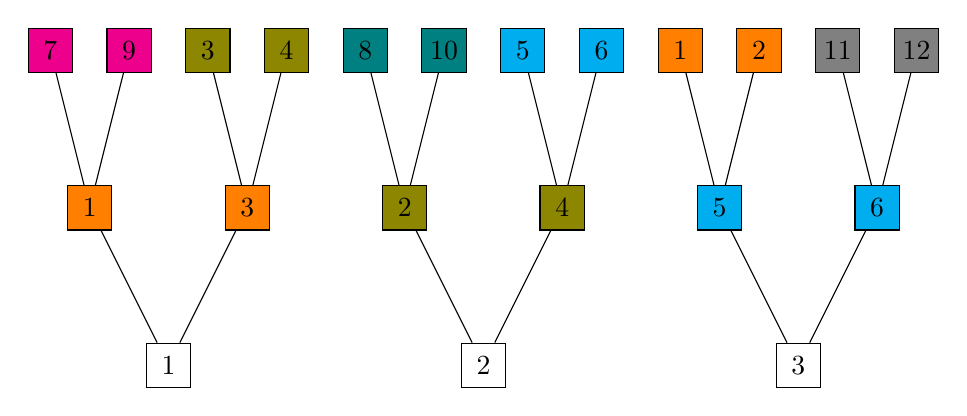
\begin{tikzpicture}
  \tikzstyle{node}=[rectangle,draw, minimum width=16pt, minimum height=16pt, inner sep=0pt, fill=white]
  \tikzstyle{color1}=[fill=orange]
  \tikzstyle{color2}=[fill=olive]
  \tikzstyle{color3}=[fill=cyan]
  \tikzstyle{color4}=[fill=magenta]
  \tikzstyle{color5}=[fill=teal]
  \tikzstyle{color6}=[fill=gray]

  \node[node, color4] (01)  at (-5.5, 2) {$7$};
  \node[node, color4] (02)  at (-4.5, 2) {$9$};
  \node[node, color2] (03)  at (-3.5, 2) {$3$};
  \node[node, color2] (04)  at (-2.5, 2) {$4$};
  \node[node, color5] (05)  at (-1.5, 2) {$8$};
  \node[node, color5] (06)  at (-0.5, 2) {$10$};
  \node[node, color3] (07)  at (0.5,  2) {$5$};
  \node[node, color3] (08)  at (1.5,  2) {$6$};
  \node[node, color1] (09)  at (2.5,  2) {$1$};
  \node[node, color1] (010) at (3.5,  2) {$2$};
  \node[node, color6] (011) at (4.5,  2) {$11$};
  \node[node, color6] (012) at (5.5,  2) {$12$};

  \node[node, color1] (11) at (-5, 0) {$1$};
  \node[node, color1] (12) at (-3, 0) {$3$};
  \node[node, color2] (13) at (-1, 0) {$2$};
  \node[node, color2] (14) at (1,  0) {$4$};
  \node[node, color3] (15) at (3,  0) {$5$};
  \node[node, color3] (16) at (5,  0) {$6$};

  \node[node] (21) at (-4, -2)  {$1$};
  \node[node] (22) at (0,  -2)  {$2$};
  \node[node] (23) at (4,  -2)  {$3$};

  \path (21) edge (11);
  \path (21) edge (12);
  \path (22) edge (13);
  \path (22) edge (14);
  \path (23) edge (15);
  \path (23) edge (16);
  \path (11) edge (01);
  \path (11) edge (02);
  \path (12) edge (03);
  \path (12) edge (04);
  \path (13) edge (05);
  \path (13) edge (06);
  \path (14) edge (07);
  \path (14) edge (08);
  \path (15) edge (09);
  \path (15) edge (010);
  \path (16) edge (011);
  \path (16) edge (012);
\end{tikzpicture}
}
\caption[Pooling auf Graphen]{Illustration einer Pooling-Operationen der Größe $4$ (\bzw{} zweier Pooling-Operationen der Größe $2$) auf einem Graphen \gls{G} der Größe $\left|\gls{V}\right| = 8$.
Das Clustering von \gls{G} liefert uns im ersten Schritt $N_1 =\left|\gls{V}_1\right| = 5$ Knoten und im darauf folgenden $N_2 = \left|\gls{V}_2\right| = 3$ Knoten.
Die Größen der Graphen werden daraufhin zu $N_2 = 3$, $N_1 = 6$ und $N_0 = 12$ angepasst, so dass jeder Knoten auf genau $2$ Vorgängerknoten verweist, indem \enquote{Fake}-Knoten zu $\gls{G}_1$ (1 Knoten) und $\gls{G}_0$ (4 Knoten) hinzugefügt werden.
Mit der Anordnung der Knoten zu einem binären Baum (d) kann die Pooling-Operation $\max\left(\cdot\right)$ eines Signals $\ve{f} \in \gls{R}^{12}$ auf $\gls{G}_0$ dann effizient als $\ve{f}_{\mathrm{pool}} \coloneqq {\left[ \max\left(\ve{f}_1, \ve{f}_2, \ve{f}_3, \ve{f}_4 \right), \max\left(\ve{f}_5, \ve{f}_6, \ve{f}_7, \ve{f}_8 \right), \max\left(\ve{f}_9, \ve{f}_{10}, \ve{f}_{11}, \ve{f}_{12} \right) \right]}^{\top} \in \gls{R}^3$ implementiert werden, wobei die Werte der \enquote{Fake}-Knoten $\ve{f}_2, \ve{f}_6, \ve{f}_{11}, \ve{f}_{12}$ auf den neutralen Wert $0$ der \gls{relu}-Aktivierungsfunktion gesetzt werden.}
\label{fig:pooling}
\end{figure}


Nach jedem Vergröberungsschritt besitzt ein Knoten entweder genau einen oder zwei Kinder, je nachdem ob es zum Zeitpunkt der Betrachtung noch einen unmarkierten Nachbarn gibt.
Falls ein Knoten \gls{v} im Graphen $\gls{G}_{l+1}$ nur ein Kind besitzt, so wird ein \emph{Fakeknoten} ohne Kanten in den Graphen $\gls{G}_l$ hinzugefügt~\cite{Defferrard}.
Damit besitzt jeder Knoten folglich nun immer zwei Kinder.
Foglich kann über die Eltern-Kind-Beziehung von der $L$-ten bis zur $0$-ten Stufe ein balancierter, binärer Baum aufgebaut werden.
Reguläre Knoten aus dem Graphen besitzen damit entweder (a) genau zwei reguläre Knoten, (b) einen regulären Knoten und einen Fakeknoten als Kinder und (c) Fakeknoten besitzen immer genau zwei Fakeknoten als Kinder~\cite{Defferrard}.
Abbildung~\ref{fig:pooling} illustriert die Konstruktion eines solchen Baumes.
Die Merkmale an den Fakeknoten eines Graphen werden mit einem neutralen Wert initialisiert, \dhe{} \zB{} mit Null bei einem Netz mit \gls{relu}-Aktivierungsfunktion und der Verwendung von Max-Pooling als Poolingoperation~\cite{Defferrard}.
Ebenso kann auf diesen Fakeknoten weiterhin ohne Einschränkungen gefaltet werden, da sie keinerlei Nachbarknoten besitzen.
Die Anordnung der Knoten zu einem balancierten, binären Baum liefert uns eine Ordnung auf den Knoten von $\gls{G}_0$ bis $\gls{G}_{L-1}$, auf der wir eine Poolingoperation völlig analog zu einem eindimensionalen Gitter mit einer Größe und Schrittweise von zwei definieren können~\cite{Defferrard}.
Diese Anordnung der Knoten macht den Prozess des Poolings extrem effizient und erlaubt ebenso eine parallele Verarbeitungsarchikektur auf GPUs~\cite{Defferrard}.

Größere Poolinggrößen müssen ein Vielfaches von zwei sein und können dann ebenso leicht über eine tieferstufigere Vergröberung implementiert werden (\vgl{} Abbildung~\ref{fig:pooling}).

\subsection{Erweiterung auf Graphen im zweidimensionalen Raum}
\label{pooling_erweiterung}

Sei $\gls{G}_l = \left(\gls{V}_l, \gls{E}_l, \gls{p}_l\right)$ ein Graph im zweidimensionalen euklidischen Raum, wobei die Position der Knoten des Graphen eindeutig über die Funktion $\gls{p}_l \colon \gls{V}_l \to \gls{R}^2$ bestimmt ist (\vgl{} Kapitel~\ref{graphrepraesentationen_von_bildern}).
Dann lässt sich der mehrstufige Clusteralgorithmus Graclus aus Kapitel~\ref{graphvergroeberung} insofern anpassen, dass dieser die Vergröberung eines Graphen auch in Bezug auf die Position seiner Superknoten in der Ebene wiederspiegelt.
Sei dafür weiterhin $\gls{v}^* \coloneqq \left\{ \gls{v}_i, \gls{v}_j \right\} \in \gls{V}_{l+1}$, ein Superknoten der Knoten $\gls{v}_i, \gls{v}_j \in \gls{V}_l$.
Dann ergibt sich die neue Position von $\gls{v}^*$ als
\begin{equation*}
  \gls{p}_{l+1}\left(\gls{v}^*\right) \coloneqq \frac{\gls{p}_l\left(\gls{v}_i\right) + \gls{p}_l\left(\gls{v}_j\right)}{2}.
\end{equation*}
Für Superknoten $\gls{v}^* \coloneqq \left\{\gls{v}_i\right\} \in \gls{V}_{l+1}$ mit einem einzigen Knoten $\gls{v}_i \in \gls{V}_l$ bleibt die Position unverändert mit $\gls{p}_{l+1}\left(\gls{v}^*\right) \coloneqq \gls{p}_l\left(\gls{v}_i\right)$.
Die Adjazenzmatrizen $\gls{Adist} \in {\left[0, 1\right)}^{N \times N}$ und $\gls{Arad} \in {\left[0, 2\pi\right]}^{N \times N}$ zu $\gls{G}_{l+1}$ können dann analog zu Kapitel~\ref{graphrepraesentationen_von_bildern} aus $\gls{V}_{l+1}$, $\gls{E}_{l+1}$ und $\gls{p}_{l+1}$ gewonnen werden.

Wohnt den Knoten in $\gls{G}_l = \left(\gls{V}_l, \gls{E}_l, \gls{p}_l, \gls{m}_l\right)$ wie in Kapitel~\ref{superpixel} zusätzlich eine Masse $\gls{m}_l \colon \gls{V}_l \to \gls{R}$ bei, so gewichtet sich die Position des Superknotens $\gls{v}^* \in \gls{V}_{l+1}$ abhängig der Massen $\gls{m}\left(\gls{v}_i\right)$ und $\gls{m}\left(\gls{v}_j\right)$ als
\begin{equation*}
  \gls{p}_{l+1}\left(\gls{v}^*\right) \coloneqq \frac{\gls{m}_l\left(\gls{v}_i\right) \gls{p}_l\left(\gls{v}_i\right) + \gls{m}_l\left(\gls{v}_j\right) \gls{p}_l\left(\gls{v}_j\right)}{\gls{m}_l\left(\gls{v}_i\right) + \gls{m}_l\left(\gls{v}_j\right)}.
\end{equation*}
Die neue Masse des Superknotens ergibt sich dann als Vereinigung der Massen $\gls{m}_{l+1}\left(\gls{v}^*\right) \coloneqq \gls{m}_l\left(\gls{v}_i\right) + \gls{m}_l\left(\gls{v}_j\right)$.
Damit erhält der vergröberte Graph $\gls{G}_{l+1}$ die Positionen und Massen seiner Vorgängerknoten des Graphen $\gls{G}_l$ im zweidimensionalen euklidischen Raum.
